% Figura 2 — Pipeline de classificacao de anomalias (NOC Lite)
% Fontes: arquitetura_sistema.md (1.2/1.3) + notas_coder.md (Sec. 0, 1.1, 2).
% Corrigido (Chris): text width + align=center nos estilos stage/cls para evitar
% truncamento nas bordas das 5 caixas superiores; quebras explicitas em tokens
% longos (extract_features_from_db, tokenise_metrics); DDOS_ATTACK forçado para
% linha propria apos "=>".
\documentclass[tikz,border=4pt]{standalone}
\usepackage{tikz}
\usepackage{amssymb}
\newcommand{\gr}{\mathrel{>}}
\newcommand{\gequal}{\mathrel{\geq}}
\usetikzlibrary{arrows.meta,positioning,shapes.geometric,decorations.pathreplacing}
\begin{document}
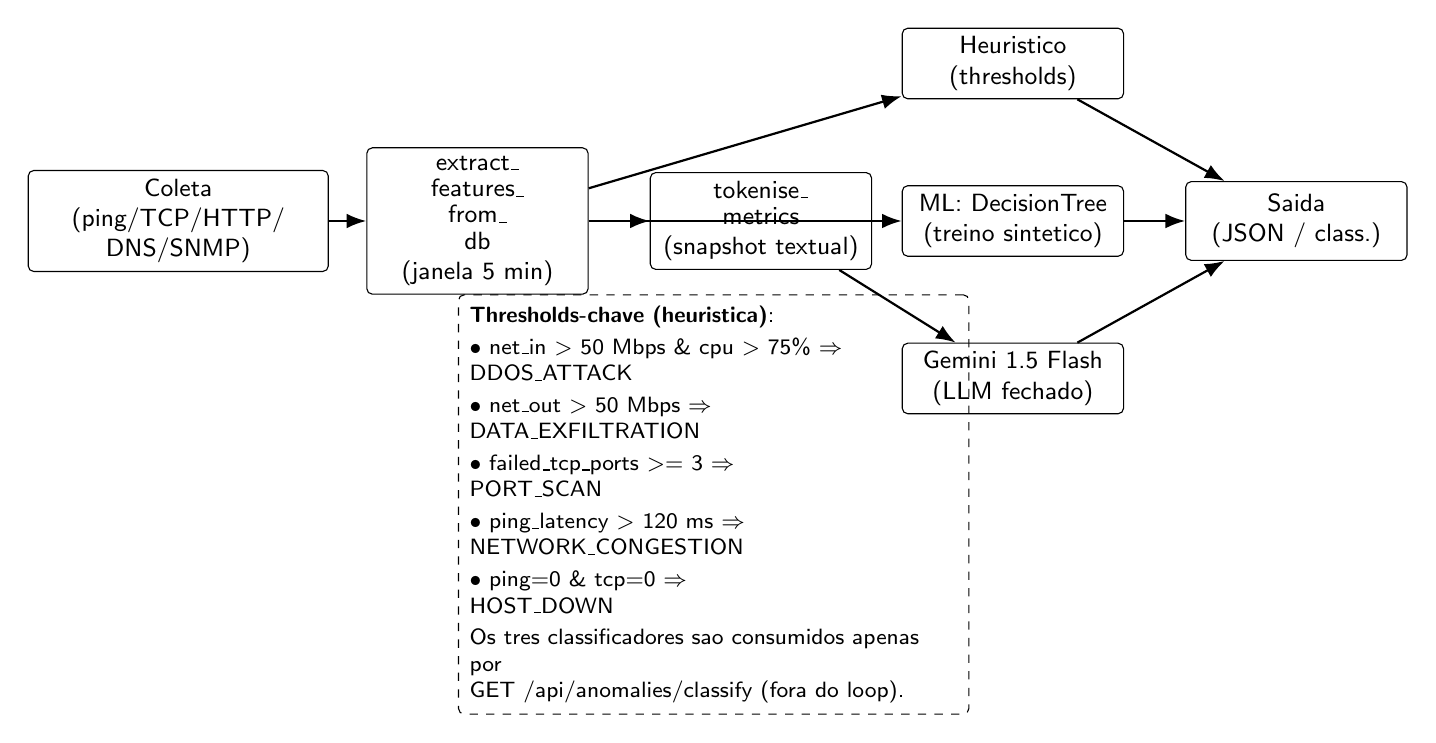
\begin{tikzpicture}[
    font=\sffamily\small,
    box/.style={rectangle, draw=black, rounded corners=2pt,
                minimum width=2.8cm, minimum height=0.9cm,
                text width=2.6cm, align=center, fill=white, inner sep=3pt},
    stage/.style={rectangle, draw=black, rounded corners=2pt,
                  minimum width=2.8cm, minimum height=1.0cm,
                  text width=2.6cm, align=center, fill=white, inner sep=3pt},
    cls/.style={rectangle, draw=black, rounded corners=2pt,
                minimum width=2.8cm, minimum height=0.8cm,
                text width=2.6cm, align=center, fill=white, inner sep=3pt},
    arrow/.style={-{Latex[length=2.5mm]}, thick, draw=black},
    darrow/.style={-{Latex[length=2.5mm]}, thick, draw=black, dashed},
  ]

  % Coleta
  \node[stage, text width=3.6cm, minimum width=3.6cm] (col) at (0,0) {Coleta\\(ping/TCP/HTTP/\\DNS/SNMP)};
  \node[stage] (ext) at (3.8,0) {extract\_\\[-1.5pt]features\_\\[-1.5pt]from\_\\[-1.5pt]db\\(janela 5 min)};
  \node[stage] (tok) at (7.4,0) {tokenise\_\\[-1.5pt]metrics\\(snapshot textual)};

  % Classificadores (paralelos)
  \node[cls] (h)  at (10.6, 2.0) {Heuristico\\(thresholds)};
  \node[cls] (m)  at (10.6, 0.0) {ML: DecisionTree\\(treino sintetico)};
  \node[cls] (g)  at (10.6,-2.0) {Gemini 1.5 Flash\\(LLM fechado)};

  % Saida
  \node[stage] (out) at (14.2,0) {Saida\\(JSON / class.)};

  % Fluxos
  \draw[arrow] (col) -- (ext);
  \draw[arrow] (ext) -- (tok);
  \draw[arrow] (ext) -- (h);
  \draw[arrow] (ext) -- (m);
  \draw[arrow] (tok) -- (g);
  \draw[arrow] (h) -- (out);
  \draw[arrow] (m) -- (out);
  \draw[arrow] (g) -- (out);

  % --- Anotacao de thresholds (chaves) ---
  \node[rectangle, draw=black, dashed, rounded corners=2pt,
        text width=6.2cm, inner sep=4pt, font=\sffamily\footnotesize, align=left]
        at (6.8,-3.6) {
        \textbf{Thresholds-chave (heuristica)}:\\[2pt]
        $\bullet$ net\_in \textgreater{} 50 Mbps \& cpu \textgreater{} 75\% $\Rightarrow$\\ DDOS\_ATTACK\\[2pt]
        $\bullet$ net\_out \textgreater{} 50 Mbps $\Rightarrow$\\ DATA\_EXFILTRATION\\[2pt]
        $\bullet$ failed\_tcp\_ports \textgreater{}= 3 $\Rightarrow$\\ PORT\_SCAN\\[2pt]
        $\bullet$ ping\_latency \textgreater{} 120 ms $\Rightarrow$\\ NETWORK\_CONGESTION\\[2pt]
        $\bullet$ ping=0 \& tcp=0 $\Rightarrow$\\ HOST\_DOWN\\[2pt]
        Os tres classificadores sao consumidos apenas por\\
        GET /api/anomalies/classify (fora do loop).
        };
\end{tikzpicture}
\end{document}
